\chapter{Literature review}\label{cap:literature}

This chapter provides an overview of the current state of literature on a variety of subjects related to the thesis.
Its main goals are to provide the reader with context for the research described here and to highlight the research gap that the work tries to address.
Where appropriate, references for in-depth materials on topics that are out of scope of this work are provided.

\section{Remote sensing for forestry applications}

As was mentioned in the introduction, remote sensing is widely used for extending labor-intensive and time-consuming manual forest inventories.
This is especially relevant in countries where massive areas are covered by forests, such as Russia, Brazil, Canada, USA, and China, which are the top five countries for forest area according to \cite{GlobalForestResources2020}.
This section provides examples of various remote sensing techniques used in various forestry applications, before going in more detail into specifically UAV LiDAR and RGB, which are the focus of the described framework.

\cite{sinica-sinavskisForestStandVolume2022} combines LiDAR point clouds with Sentinel-2 images to predict timber volume on a stand level.
They use an unusual approach, using Sentinel-2 images for species detection by clustering, LiDAR point clouds for estimating tree counts and average tree heights, and combining them into to variables used to fit the final regression models.
The reported relative RMSE values are 14-22\%, with errors larger for deciduous tree species.

\cite{ferrariFusingSentinel1Sentinel22023} use Fully Convolutional Networks \cite{longFullyConvolutionalNetworks2015} for fusion of optical Sentinel-2 and SAR Sentinel-1 data.
They show that the fusion approach outperforms single modality approaches, especially when there is any cloud cover present.

LiDAR has been used for forestry applications for a long time with publications on the topic dating back 40 years.
\cite{nelsonDeterminingForestCanopy1984} is one of the earliest studies that explores usage of airborne LiDAR for measuring forest canopy profiles and estimating tree heights and canopy closure (a measure of forest canopy coverage that indicates what proportion of the sky is obscured by the tree crowns when viewed from the ground).

\cite{nilssonEstimationTreeHeights1996, naessetDeterminationMeanTree1997, naessetEstimatingTimberVolume1997, carson2004lidar}.

\section{Machine learning and deep learning on point clouds}\label{sec-ml-dl}

The reader is assumed to be familiar with general concepts of machine learning and deep learning.
For an introduction or a refresher, one of the best resources is \cite{goodfellowDeepLearning2016}.
For a more detailed exploration, \cite{wangRecentAdvancesDeep2020} offers a selection of papers on topics relevant to modern deep learning techniques.
The section is focused on providing a short overview of machine learning and deep learning for point clouds, as LiDAR point clouds are the main source of data for the framework described in this thesis and point clouds are in general a less well-known modality in machine learning than images or text.

Classic machine learning approaches rely on manual feature preparation.
Two main groups of tasks are per-point predictions, which is in many ways similar to the task of semantic segmentation of images, that requires per-point features, and per-cloud predictions that either process entire point clouds or individual segments, separated be some preprocessing routine.
\cite{weinmannFeatureRelevanceAssessment2013} show that careful selection of features is crucial for accurate and efficient interpretation of point cloud data.
They also provide definitions of some of the most used manual features that aim to describe the 3D structure of point sets.
The features are based on combinations of eigenvalues of a local covariance matrix of a set of points.
They can be calculated on a per-point basis by using fixed-size or nearest-neighbor neighborhoods, or for whole segments of point clouds.
The used features were originally introduced \cite{westContextdrivenAutomatedTarget2004}, \cite{paulyEfficientSimplificationPointsampled2002}, and \cite{malletRelevanceAssessmentFullwaveform2011}, and include linearity, planarity, and scatter, aiming to indicate the presence of a linear, planar, or volumetric structures, and also omnivariance, anisotropy, eigentropy, the sum of eigenvalues, and curvature.
The formulas for the features are provided in Section~\ref{sec-training-tree-processors} where they are used for training parameter prediction models for segmented trees.

\cite{belloReviewDeepLearning2020} and \cite{guoDeepLearning3D2021} offer detailed reviews of the deep learning approaches used in various problems related to processing point clouds.
Below is a very short summary.

The first model to work directly work on point clouds is the PointNet \cite{qiPointNet2017}.

\begin{figure}
\centering{
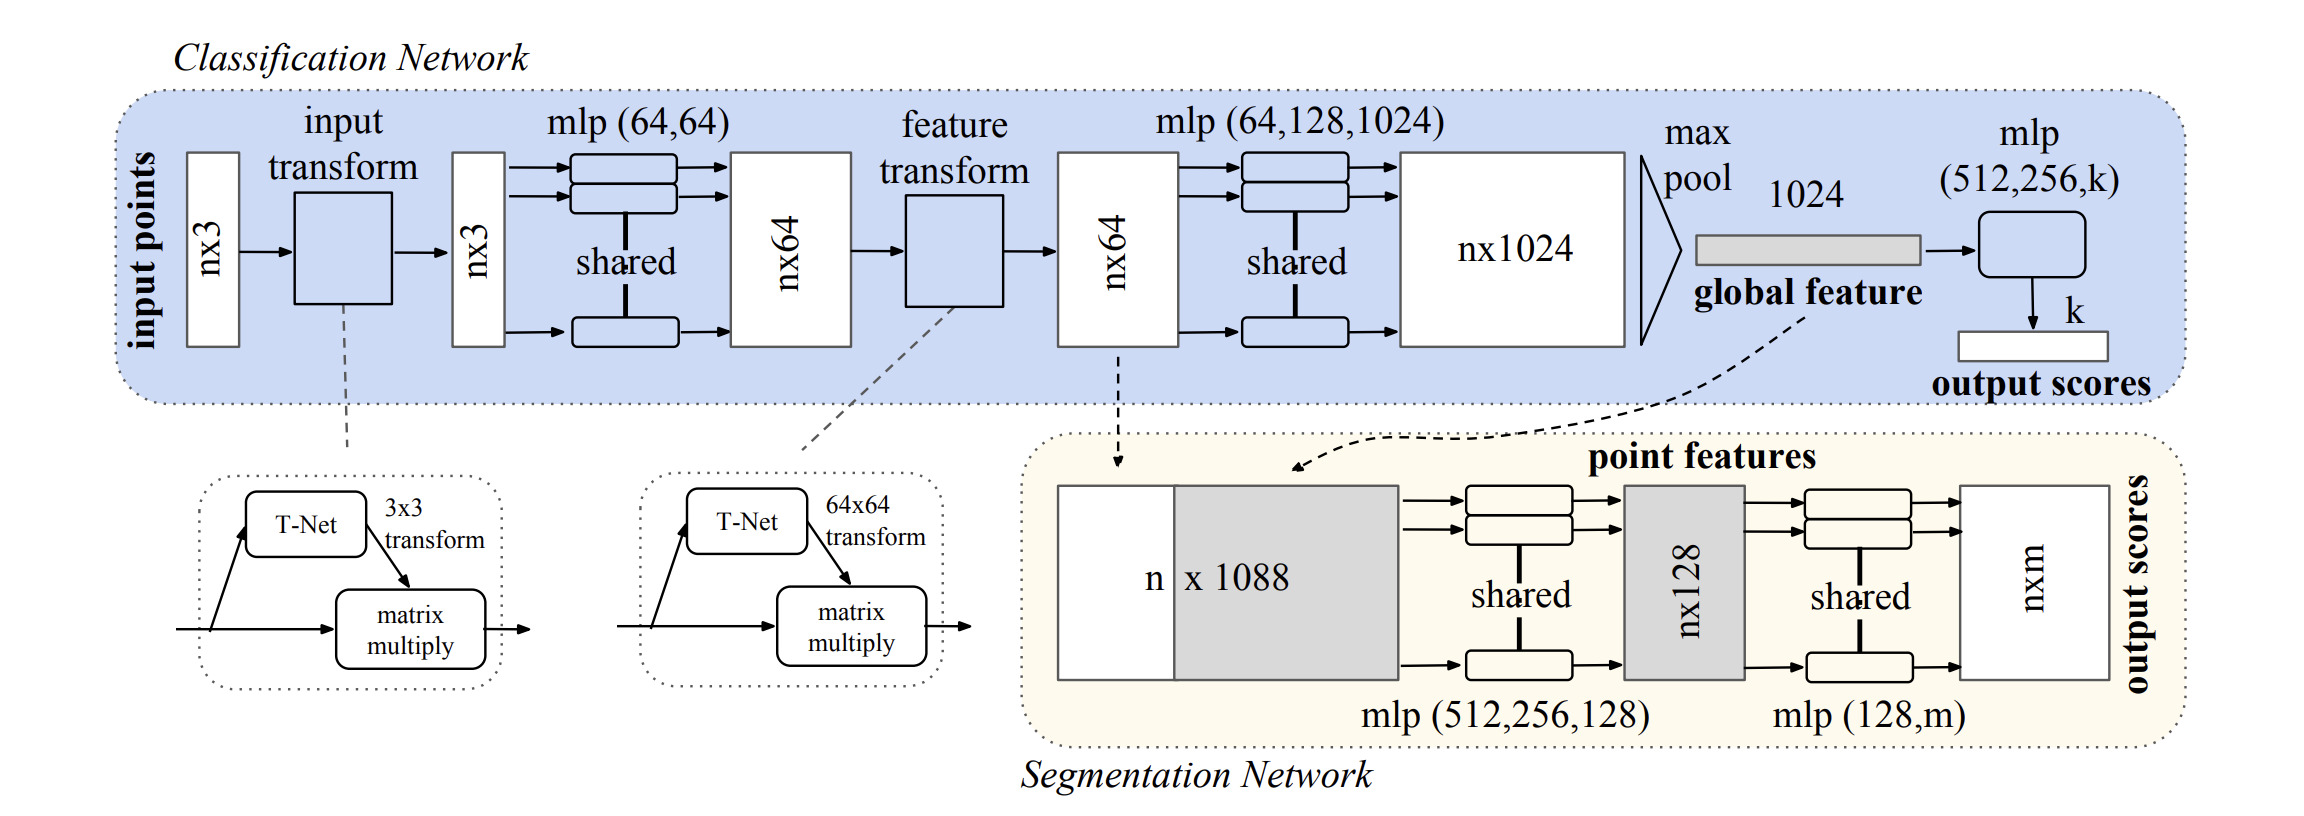
\includegraphics[width=\textwidth]{../images/pointnet_architecture.jpg}
}
\caption{\label{fig-pointnet-architecture}PointNet architecture. Figure
from (Qi, Su, et al. 2017)}
\end{figure}

PointNet++ \cite{qiPointNetPlusPlus2017} addresses the drawbacks of the original PointNet model, namely only two scales for feature caclulation.
It introdcuces hierarchical feature learning by consecutive application of set abstraction modules

\begin{figure}
\centering{
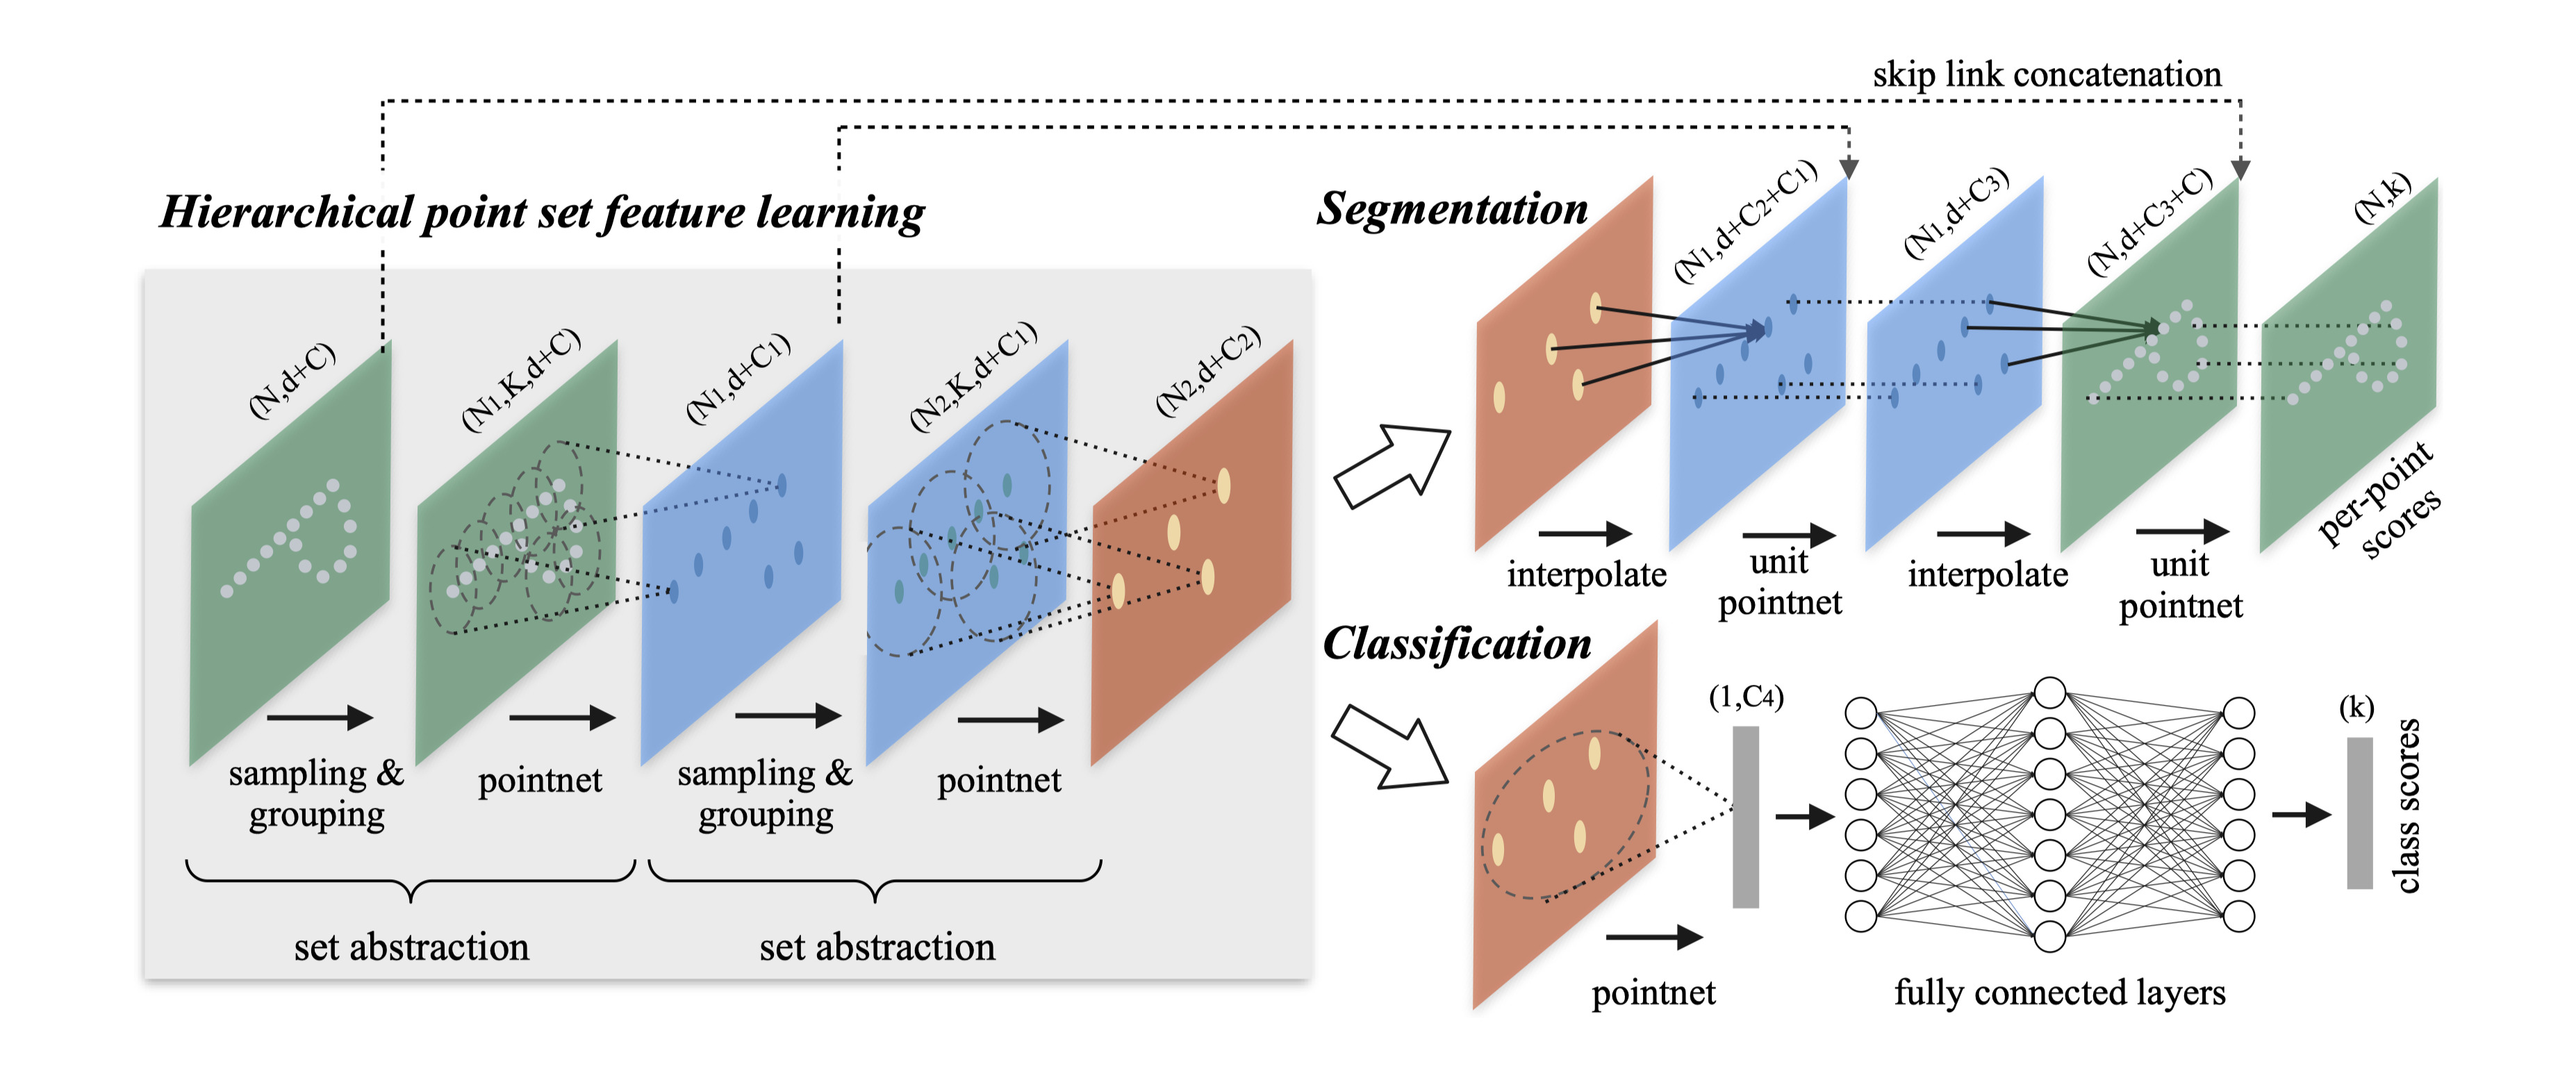
\includegraphics[width=\textwidth]{../images/pointnet2_architecture.jpg}
}
\caption{\label{fig-pointnet2-architecture}PointNet++ architecture.
Figure from (Qi, Yi, et al. 2017)}
\end{figure}

\section{Area-based approach}\label{sec-area-based-approach}

The most common way to use LiDAR for mapping forest attributes is the area-based approach \cite{whiteABAGuide2013}.
Figure~\ref{fig-aba-schema} shows its schematic representation.
It consists of a LiDAR survey covering the whole area of interest and a manual forest inventory providing ground truth data for fitting statistical models and validating the results.
The inventory usually consists of many circular ground plots with every tree within counted and attributes of interest either directly measured or calculated and averaged.
The point cloud is clipped by the extents of the ground plots, and for each plot it is reduced to a collection of manually selected metrics.
The metrics usually include descriptions of the height distribution of the points, but often reflection intensities and other sensor-provided information is used as well, such as the return number, the number of returns, etc. (a brief discussion on the use of intensity-based features can be found in Section~\ref{sec-intensity-based-features}).
In general, any summary statistic that can be derived from a collection of points can be used, including features mentioned in Section~\ref{sec-ml-dl}.
These metrics are then used as input features for fitting regression and classification models to predict the forest attributes measured on the corresponding plots.
The same metrics are calculated for the entire area of interest, using a grid with a cell size similar in area to the area of a single ground plot.
The models are then applied to the grid, generating an extrapolation of the required attributes.

\begin{figure}
\centering{
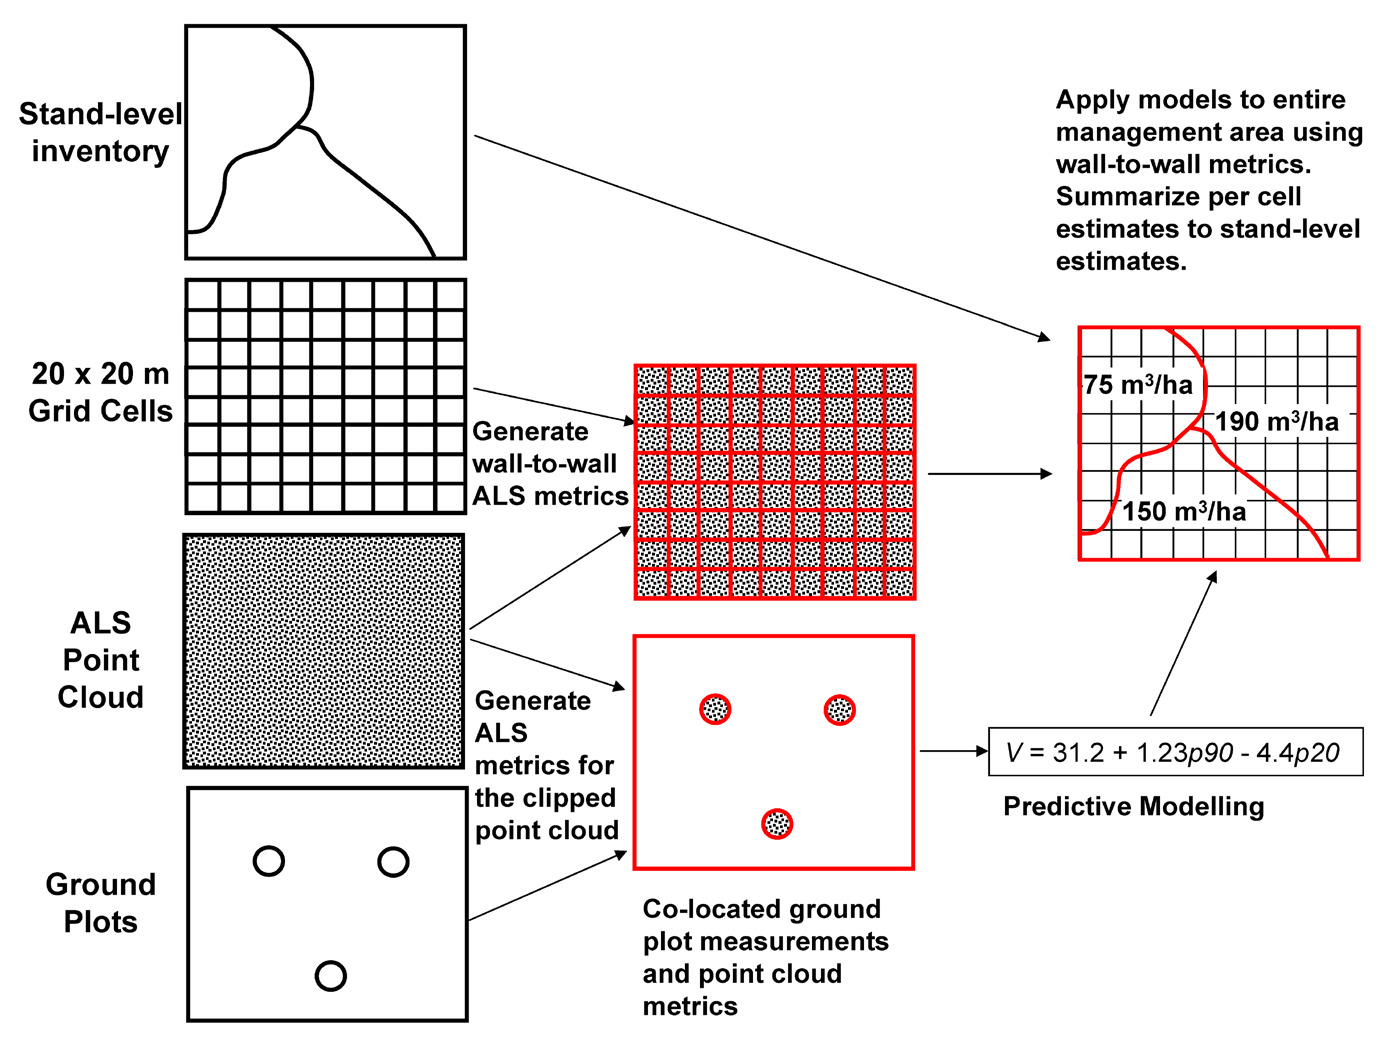
\includegraphics[width=\textwidth]{../images/aba_schematic.jpg}
}
\caption{\label{fig-aba-schema}Area-based approach schematic. Figure
from (White et al. 2013)}
\end{figure}

Area-based approach is extensively used both in research and in industry because it provides many advantages.
It is relatively easy to implement.
In fact, basic familiarity with the R programming language is enough to create your own area-based approach pipelines since a full, scalable implementation exists in the `lidR` package \cite{rousselLidRPackage2020}.
It is also straightforward to extend with other data sources such as satellite or aerial images, and it works even with sparse data: for successful plot and stand level modeling point densities as low as 0.5 points per square meter have been reported to be enough \cite{treitzLiDARSamplingDensity2012, jakubowskiTradeoffsLidarPulse2013}.
Still, it requires a lot of field inventory data to work, since every ground plot becomes a single example for the models.
The models that can be used are also relatively simple, because of how expensive the data collection is.
Data-hungry approaches like neural networks usually don't have enough data to train.
The results are also very coarse – predicted on a grid with the size defined by the area of a plot (a common plot shape is a circle with 9-meter radius, which is approximately equivalent to a square grid cell with 16-meter side).
This is why they are usually further aggregated to stand level.

\cite{bouvierGeneralizingPredictiveModels2015}

\cite{zhangImprovedAreabasedApproach2023} use a modification of the area-based approach to predict plot-level diameter at breast height (dbh) by utilizing known allometric dependencies between tree height as a hypothesis set for fitting statistical models.
They use airborne LiDAR measurements with an average density of 9.6 points per square meter and report a relative error of 11%.

\cite{vermeerLidarbasedNorwegianTree2023} uses a U-Net \cite{ronnebergerUNetConvolutionalNetworks2015} image semantic segmentation model on LiDAR-derived 1-meter resolution digital terrain models and canopy height maps to predict the distribution of three main tree species in a Norwegian forest.
They achieve a macro $F_1$ of 0.70 when including the background class, and 0.63 when including only the target species classes, as evaluated on independent field inventory plots.

\cite{kcEstimationAboveGroundForest2024}

\section{Individual tree-based approach}\label{sec-individual-tree-approach}

\cite{liNewMethodSegmenting2012} developed a well performing algorithmic method for segmentation of individual tree crowns in LiDAR point clouds for coniferous forests that relies on the pointy shape characteristic of many coniferous species and segments the trees from top to bottom.

\cite{lucasIdentificationLinearVegetation2019} uses the set of eigenvalue-based features calculated for each point in a fixed-radius neighborhood, with other geometrical features including maximum local height difference and height standard deviation, local radius and local point density.
They also use two point-based features that don't rely on a neighborhood: the number of returns and the normalized return number, proposed in \cite{guoRelevanceAirborneLidar2011}.
They use Random Forest to separate the points that belong to vegetation after first removing the planar features corresponding to grass, soil, and water surfaces.

\subsection{Image-only}

Many approaches rely only on images, mostly RGB and multispectral ones.
The main advantage of such approaches is a well-established and well-known toolbox in terms of both algorithmic processing and deep learning, as many of the most important deep learning milestones were achieved in the field of computer vision.
The main disadvantages were briefly mentioned in the introduction.
Passive sensors rely on the sun as the source, and thus greatly depend on lightning such as cloud and terrain shadows, time of day, season.

\cite{lassalleDeepLearningbasedIndividual2022} used high-resolution satellite imagery.

\cite{weinsteinDeepForestPythonPackage2020} is a Python package for image-based tree detection.

\cite{oscoConvolutionalNeuralNetwork2020} use a convolutional neural network on UAV multispectral images to count citrus trees in an orchard by predicting a confidence map that shows the likelihood of each pixel containing a tree.
They report $F_1$-scores of up to 0.95

\cite{venturaIndividualTreeDetection2024} built a network they call HR-SFAnet, consisting of a VGG-16 \cite{simonyanVeryDeepConvolutional2014} backbone feature extractor, a confidence head, and a parallel attention head, which is a deeper modification of the SFANet proposed in \cite{zhuDualPathMultiScale2019} for counting the amount of people in photos, for detecting individual trees in urban environments using high-resolution multispectral images.
They report $F_1$-scores of 0.75, with average positioning error of 2.2 meters.

\subsection{Fusion of data}

\cite{liFusionApproachesIndividual2023}

\cite{balestraLiDARDataFusion2024} offers a review of 151 publications concerning fusion of LiDAR data with other remote sensing data.
The authors report that in most cases fusion improves the results.

\cite{ferreiraImprovingUrbanTree2024} use a U-Net semantic segmentation model for fusion of VNIR images and UAV LiDAR-derived feature maps including surface normals of the canopies, reflection intensities, canopy heights, and leaf-area index for mapping tree species in urban tropical areas.
Their results show that adding LiDAR-based features improves $F_1$-scores across all considered species, with average $F_1$-score 84.1.
They also use the segment anything model \cite{Kirillov_2023_ICCV} to automatically segment tree crowns with outstanding 98% boundary $F_1$-score.

\subsection{Terrestrial LiDAR}

Terrestrial LiDAR surveys usually provide very dense and detailed point clouds.
Most importantly for the task of localizing individual trees, terrestrial measurements always capture the trunks of the trees clearly.
Tree trunks are very useful for tree detection and segmentation, and there are many algorithms that use bottom-to-top approaches that trace the trunks into the canopies.

\cite{nurunnabiDevelopmentPreciseTree2024} offers a compelling example of how such detailed data can be used to provide very detailed analyses on tree level.
The authors report high accuracies on the task of segmenting the point clouds

\cite{allenTreeSpeciesClassification2022} - classifying manually extracted terrestrial LiDAR point clouds of individual trees using multi-view representation based on \cite{goyalRevisitingPointCloud2021} and a convolutional network ResNet \cite{heDeepResidualLearning2016}.

\cite{lopezserranoArtificialIntelligencebasedSoftware2022} describes a framework for fully automatic processing of terrestrial LiDAR point clouds based on trunk detection.

\cite{vianaTimberVolumeEstimation2022} use a small dataset to compare tree-level inventory metrics extracted from a terrestrial LiDAR survey and from a manual inventory.

\subsection{UAV LiDAR}

\subsubsection{CHM-based methods}

A common approach to utilize LiDAR point cloud data for tree detection is by calculating canopy height maps.

Local maxima filter – that looks at local maxima in a sliding window.
A substantial number of different tree detection algorithms are variations of the local maxima filter, differing in what the filter is applied to, how many times, with what windows, and how the results are combined or preprocessed.

Many tree-detection methods are based on construction of canopy height maps from the point clouds and applying well-known image processing techniques to work with them further.

\cite{doussExtractionIndividualTrees2022} offers an exploration of how different window size functions for the local maxima filtering applied to LiDAR-derived canopy height maps affect the quality of individual tree detection.
They show that for moderately dense forest in France, it is possible to find the parameters for the local maxima filter window that produce satisfactory results.
It is, however, clear that it requires great deal of manual adjustment, and visual inspection of the results of detection makes it clear that they are only locally consistent.
Any change in the canopy structure patterns noticeably affects the quality of the detection even for sophisticated window functions.

\cite{lisiewiczCorrectingResultsCHMBased2022} proposes a way to improve the results of CHM-based individual tree detection algorithms.